\documentclass[letterpaper]{article}
\usepackage[utf8]{inputenc}
\usepackage[spanish, mexico]{babel}
\usepackage{amssymb, amsmath}
\usepackage{stackengine}
\usepackage{graphicx}
\usepackage{ mathrsfs }
\usepackage{lipsum}
\usepackage{dsfont}
\usepackage[margin=1.5cm,
vmargin={1.5cm,0.7cm},
includefoot]{geometry}
\usepackage{setspace}
\usepackage{subcaption}
\usepackage{tocloft}
\usepackage{upgreek}
\usepackage{amsthm}
\usepackage{graphicx}
\usepackage{paralist}
\usepackage{fancyhdr}
\usepackage{lmodern}
\usepackage{tcolorbox}
\usepackage{color}
\usepackage{tikz}
\usepackage{wasysym}
\usepackage{textgreek, marvosym}
\tcbuselibrary{skins,breakable}
\pagestyle{fancy}

\renewcommand{\headrulewidth}{0.4pt}
\renewcommand{\footrulewidth}{0.4pt}

\renewcommand{\d}{\partial}

\providecommand{\abs}[1]{\left|#1\right|}
\providecommand{\norm}[1]{\left|\left|#1\right|\right|}														  
\providecommand{\pint}[1]{\langle#1\rangle}														  
\newcommand{\V}{\mathds{V}}

\newcommand{\W}{\mathds{W}}

\newtheorem*{remark}{Recuerde}

\newcommand{\F}{\mathds{F}}

\newcommand{\tq}{ \quad \cdot  \backepsilon \cdot \quad }

\newcommand{\ld}{\lim\limits_{x \to 0^{+}}}

\newcommand{\li}{\lim\limits_{x \to 0^{-}}}

\newcommand{\la}{\lim\limits_{x \to a}}

\renewcommand{\l}{\ell}

\newcommand{\R}{\mathds{R}}

\newcommand{\Po}{\mathds{P}_2(\mathds{R})}

\renewcommand{\*}{\cdot}

\makeatletter
\renewcommand*\env@matrix[1][\arraystretch]{%
	\edef\arraystretch{#1}%
	\hskip -\arraycolsep
	\let\@ifnextchar\new@ifnextchar
	\array{*\c@MaxMatrixCols c}}
\makeatother

\newtheorem{theorem}{Teorema}[]
\theoremstyle{definition}
\newtheorem{definition}{Definición}


\begin{document}
	
	\setlength{\unitlength}{1cm}
	\thispagestyle{empty}
	\begin{picture}(19,3)
	\put(-0.5,1.2){
\includegraphics[scale=.20]{img/unam1.png}}
	\put(16,1){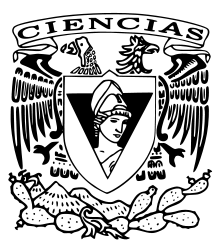
\includegraphics[scale=.29]{img/fciencias1.png}}
	\end{picture}
	
	\begin{center}
		\vspace{-114pt}
		\textbf{\large Matemáticas para las Ciencias II}\\
		\textbf{ Semestre 2020-2}\\
		Prof. Pedro Porras Flores\\
		Ayud. Irving Hernández Rosas \\
		\textbf{Tarea Examen III}\\[0.15cm]
		Kevin Ariel Merino Peña\footnote{Número de cuenta 317031326}\\ [0.12cm]
		\today
	\end{center}
	\vspace{-10pt}
	\rule{19cm}{0.3mm}
	
	\noindent Realice los siguientes ejercicios, escribiendo el procedimiento claramente. Y recuerden la tarea-examen se entregan de manera individual.\\
	
\noindent1.Sea $f: \mathbb{R} \longrightarrow \mathbb{R}$ una función diferenciable. Muestre que $u = f(y - \kappa x)$ es una solución de la ecuación diferencial parcial $$\dfrac{\partial u}{\partial x} + \kappa\dfrac{\partial u}{\partial y} = 0$$
Hagamos una observación sobre $ u $, pues debemos costruir a dicha función con el mismo dominio que f, \textit{i.e. }
\[ u(x,y) = f(y-\kappa x)  \]ahora empleemos la composición de funciones para designar una función auxiliar $ g: \R^2 \to \R $  como sigue $ g(x,y) = y-\kappa x $;
\[ u(x,y) = (f \circ g)(x,y) = f(g(x,y)) \]
luego, tomemos la derivada de $ u $ como 
\[ Du(x,y) = Df(g(x,y)) \]Veamos que, como $ g $ es una función escalar, entonces su derivada es $ \nabla g $ y por la \textbf{regla de la cadena }en funciones compuestas, tenemos que \[ D_u (x,y) = D_f(g(x,y))\nabla g \label{eq:primeraDerivada}\tag{\venus} \]donde $ \nabla g(x,y) = \left( \dfrac{\d g}{\d x}, \dfrac{\d g}{\d y} \right)= \left( -\kappa, 1 \right) $, luego de $ \ref{eq:primeraDerivada} $ tenemos que 
\begin{align*}
	D_u (x,y) &= f'(g(x,y)) \* \left( -\kappa, 1 \right)  && \text{Reemplazando lo que sabemos del gradiente}\\
	D_u (x,y) &= -f'(g(x,y))\kappa, f'(g(x,y)) && \text{Reemplazando lo que sabemos del gradiente}\\
	\dfrac{\d u}{\d x} &= -f'(g(x,y))\kappa  && \text{Derivando con respecto a }x\\
	\dfrac{\d u}{\d y} &= f'(g(x,y)) && \text{Derivando con respecto a }y\\
	\kappa\dfrac{\d u}{\d y} &= f'(g(x,y))\kappa  && \text{Multiplicando ambos miembros por el mismo real }\\
\end{align*}
\[ \dfrac{\partial u}{\partial x} + \kappa\dfrac{\partial u}{\partial y} = -f'(g(x,y))\kappa + f'(g(x,y))\kappa = 0  \]siguiendo la cadena de igualdades, tenemos que 
\[ \dfrac{\partial u}{\partial x} + \kappa\dfrac{\partial u}{\partial y} = 0 \quad \qedsymbol \]

\noindent2.Muestre que si  $u(x,y)$ y $v(x,y)$ tienen segundas parciales mixtas continuas y satisfacen las ecuaciones de 
\begin{subequations}
\label{eq:Maxwell}
Cauchy-Riemann:
\begin{align}
        \dfrac{\partial u}{\partial x} &= \dfrac{\partial v}{\partial y},         \label{eq:MaxB} \\
        \dfrac{\partial u}{\partial y} &= - \dfrac{\partial v}{\partial x}, \label{eq:MaxE}
\end{align}
\end{subequations}

Entonces ambas son armónicas.

\begin{remark}
Una función $u = u(x,y)$ con segundas derivadas parciales continuas que satisface la ecuación de Laplace  $$ \dfrac{\partial^2 u}{\partial x^2} + \dfrac{\partial^2 u}{\partial y^2}= 0,$$ se dice que es una función armónica.
\end{remark}

\noindent3. Encontrar la expansión a segundo orden de Taylor para $f(x,y) = y^2e^{-x^2}$ en $(1,1)$\\

primero hallemos las derivadas de $ f $
\begin{align*}
	\dfrac{\d}{\d x} (y^2 e^{-x^2}) &= -2xy^2e^{-x^2} &&\text{Derivando con respecto a }x\\
	\dfrac{\d}{\d y} (y^2 e^{-x^2}) &= 2ye^{-x^2} &&\text{Derivando con respecto a }y\\
	\dfrac{\d}{\d x} (-2xy^2e^{-x^2}) &= (4x^2 - 2)y^2e^{-x^2} &&\text{Derivando con respecto a }xx\\
	\dfrac{\d}{\d x} (-2xy^2e^{-x^2}) &= -4xye^{-x^2} &&\text{Derivando con respecto a }xy\\
	\dfrac{\d}{\d y} (2y^2e^{-x^2}) &= 2ye^{-x^2} &&\text{Derivando con respecto a }yy\\
\end{align*}
Luego, usando el teorema (visto en clase) sobre la expansión a segundo orden de Taylor para $ x_0 =(1,1) $ está dada por


\noindent4. Sea $f: \mathbb{R}^2 \longrightarrow \mathbb{R}$ tal que  $f(x,y) = x^2 - y^2 - xy + 5$. Encuentre los puntos críticos de $f$ y determine si son: mínimos locales, máximos locales o puntos silla.\\

\noindent5. Encuentre los valores máximos y mínimos absolutos de $f(x,y) = x^2 + 3xy + y^2 + 5$ sobre el disco unitario $\mathcal{D} = \{(x,y) \in \mathbb{R}^2 : x^2 + y^2 \leq 1 \}$\\

\noindent6. Suponga que un pentágono está compuesto por un rectángulo coronado por un triángulo isósceles (ver Figura \ref{fig:1}). Si la longitud del perímetro es fija, encuentre el área máxima posible.

\begin{figure}[h]
    \centering
    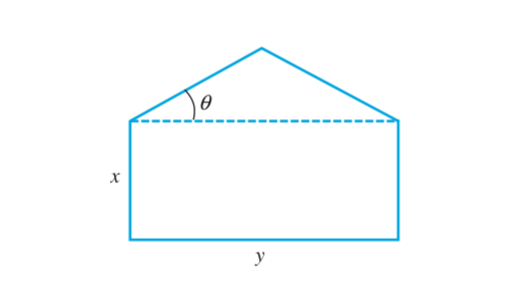
\includegraphics[width=0.5\textwidth]{img/figT}
    \caption{Maximizar el área para un perímetro dado.}
    \label{fig:1}
\end{figure}


\noindent7. Analice el comportamiento de las funciones en los puntos indicados. En la parte $b$ el análisis depende de la constante $C$.\\


a) $z = x^2 - y^2 + 3xy $ en $(0,0)$.\\
b)  $z = x^2 - y^2 + Cxy $ en $(0,0)$.




\noindent8. a) Encuentre la distancia mínima del origen en $\mathbb{R}^2$  a la superficie $z = \sqrt{x^2 - 1}$.\\

b) Haga lo mismo para la superficie $z = 6xy + 7$\\

\noindent9. Encuentre los puntos y valores críticos de las siguientes funciones sujetas a las restricciones:\\


a) $f(x,y) = x^2 - 2xy + 2y^2$, restringido a $x^2 + y^2 =1$.\\

b) $f(x,y) = \cos{(x^2 - y^2)}{}$, restringido a $x^2 + y^2 =1$.\\

c) $f(x,y) = \dfrac{x^2 - y^2}{x^2 + y^2}$, restringido a $x + y =1$.\\

d) $f(x,y) = \cos^2{x} +\cos^2{y}$, restringido a $x + y =\frac{\pi}{4}$.


\noindent10. Encuentre el máximo de la función $f(x,y) = xy$ sobre la curva $(x +1)^2 + y^2 =1$

\noindent11. Encuentre la distancia más cercana del punto $(a_1, a_2, a_3) \in \mathbb{R}^3$ al plano cuya ecuación está dada por: $b_1x_1 + b_2x_2 + b_3x_3 + b_0 = 0$, donde $(b_1, b_2, b_3) \neq 0 $

\noindent12. Encuentre el punto sobre la linea de intersección de los planos  $a_1x_1 + a_2x_2 + a_3x_3 = 0$ y $b_1x_1 + b_2x_2 + b_3x_3 + b_0 = 0$ que es más cercano al origen.

\end{document}
